\documentclass[10pt,addpoints,answers]{exam}
\usepackage{graphicx} % Required for inserting images
\usepackage{booktabs}
\graphicspath{{bilag/}}




\begin{document}
\begin{center}
{\Huge \textbf{ATLAS}}\\[0.5em]
{\LARGE Acoustic TDOA Localization and Alert System}\\[1.5em]
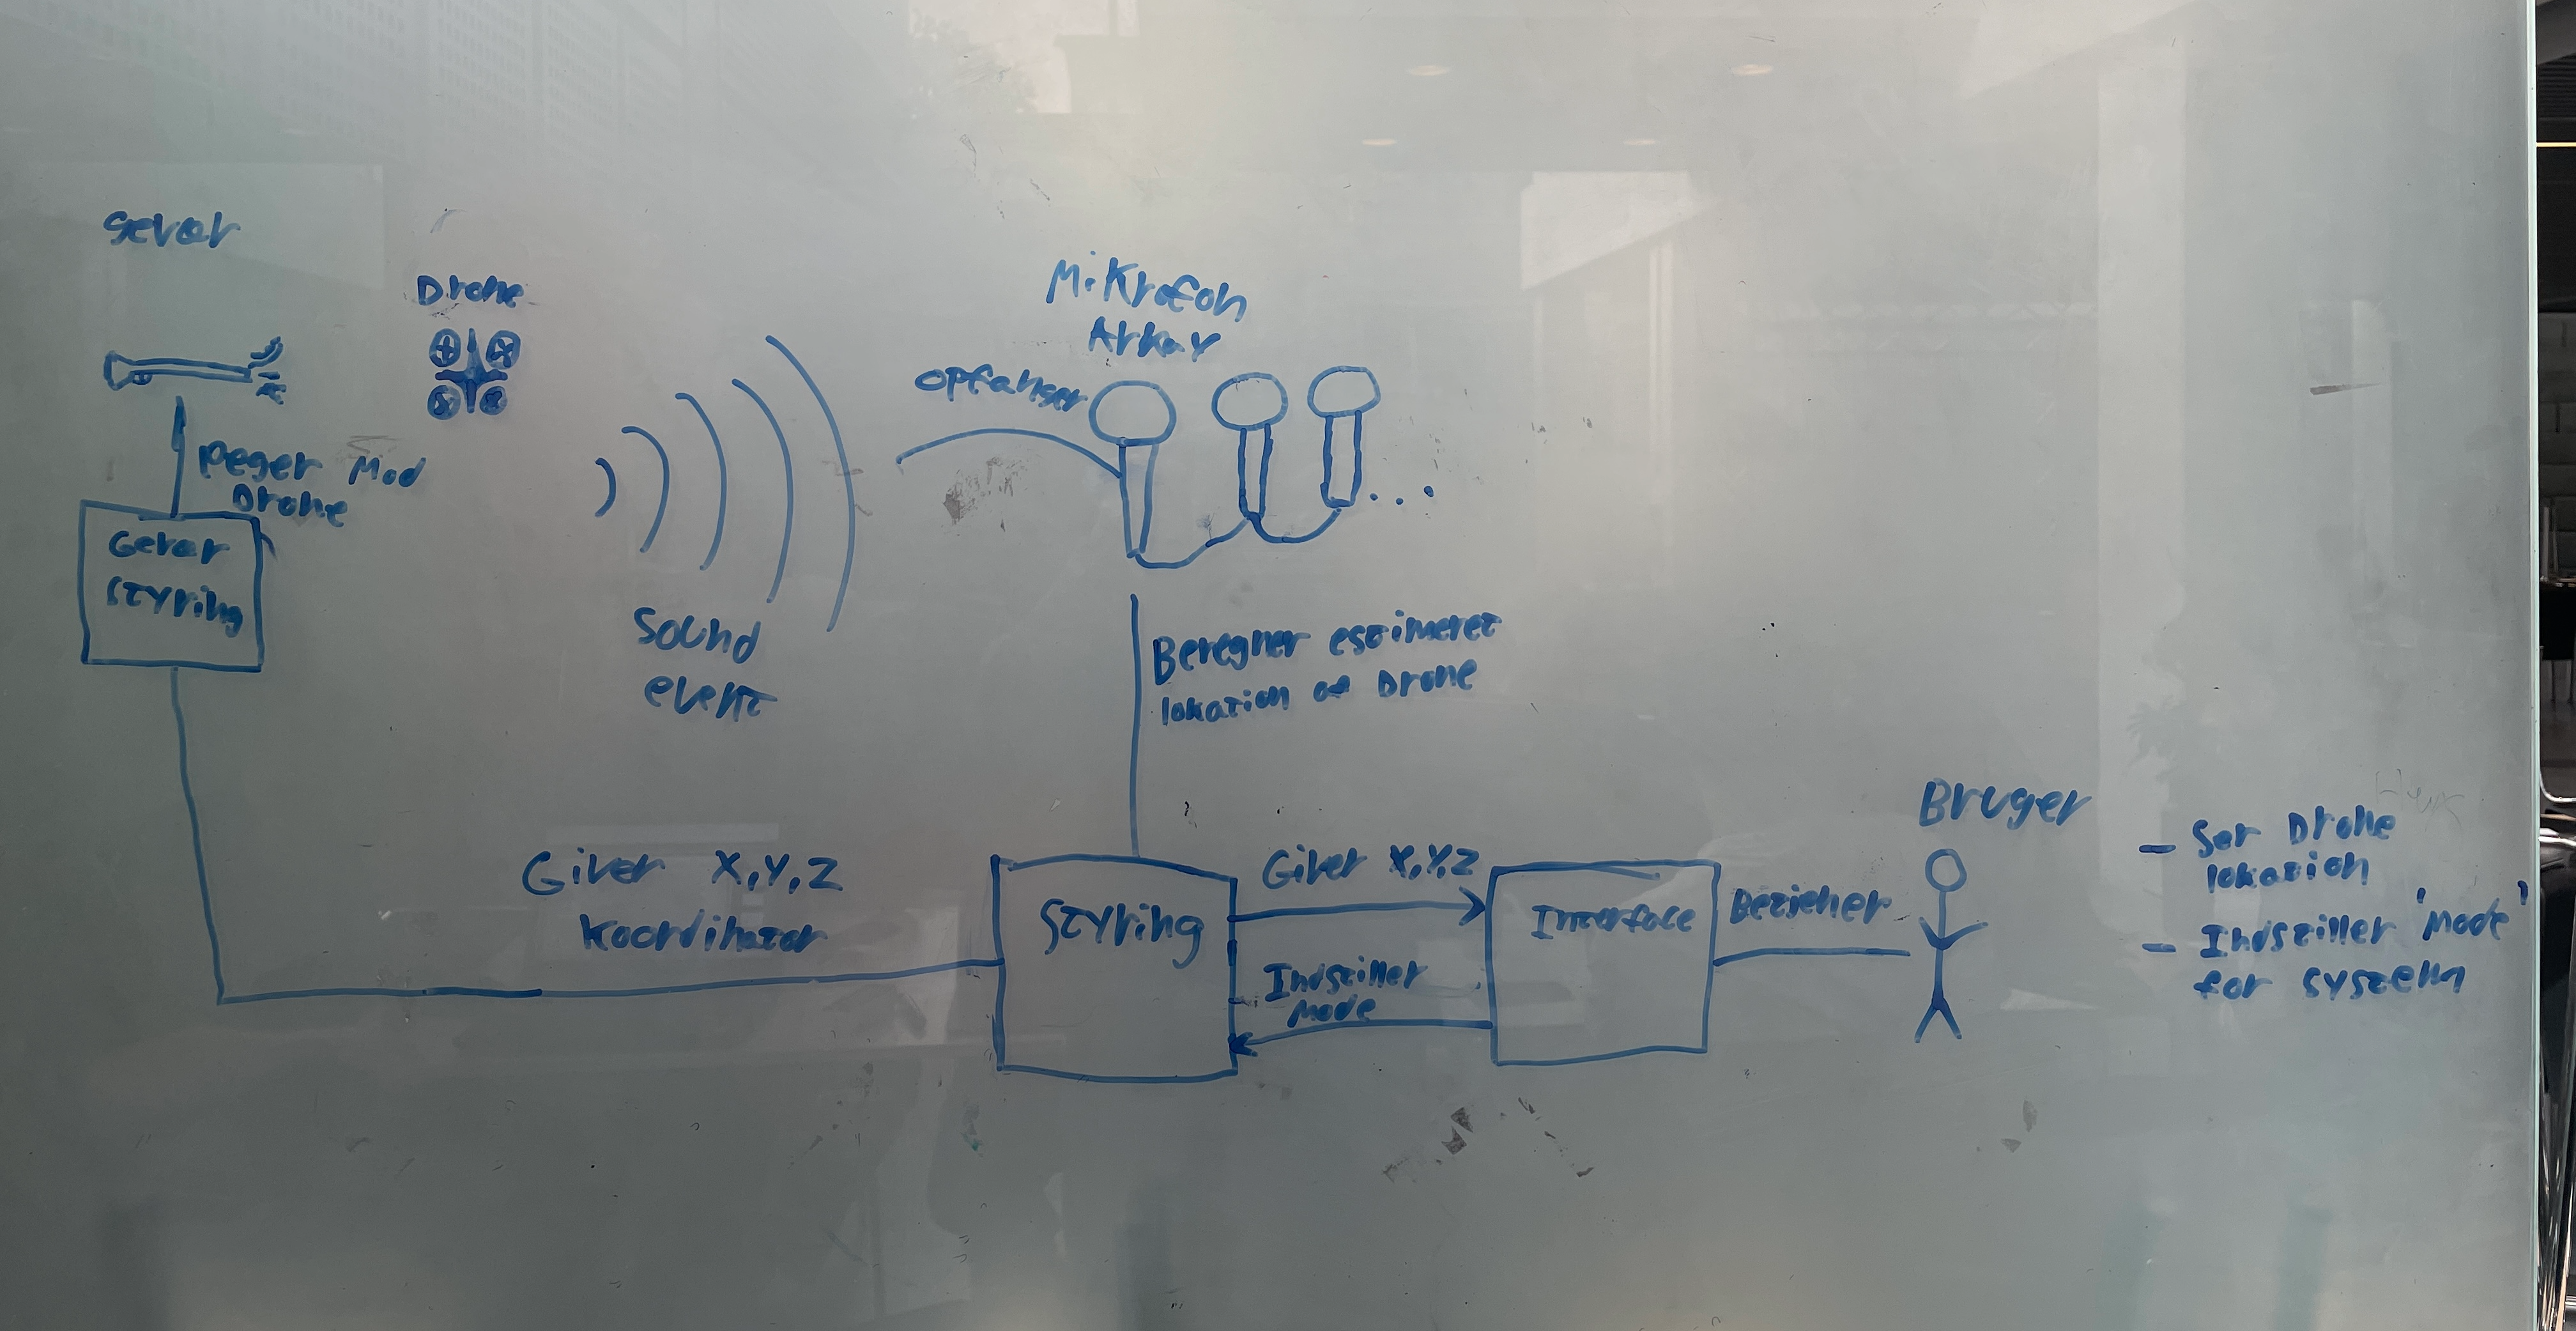
\includegraphics[width=1\linewidth]{bilag/ATLAS systemskitse.png}\\[1.5em]
{\large \textbf{\textit{Forfattere - Gruppe 5}}}\\[0.5em]
\begin{tabular}{cc}
    \toprule
    \textbf{Studienummer} & \textbf{Navn} \\
    \midrule
    202509720 & Alexander Bak Thorsen \\
    202506000 & Otto German Jørgensen \\
    202505524 & August Due Iversen \\
    202507543 & Bertram Engelbrecht Agerskov \\
    202411373 & Emil Lytzen Beck \\
    202509693 & Viktor Kirkeby Førrisdahl \\
    202411370 & Mads Sejerskilde \\
    202506410 & Frederik Buskbjerg Reichle \\
    \bottomrule
\end{tabular}\\[1.5em]
{\large \textbf{\textit{Vejleder}}}\\[0.5em]
Lars Mortensen\\[2em]

\includegraphics[width=0.2\linewidth]{bilag/ausegl_blaa.png}
\end{center}

\newpage
\section*{Projektformulering}
Verden er i forandring i dag, og nye metoder at føre krig på truer kritisk infrastruktur. Krigsførelse med droneteknologi er hurtigt blevet normen, og giver nye udfordringer på hvordan man billigt og sikkert kan beskytte luftrummet. Den danske regering havde tidligere afsat 365 milliarder kroner til oprustning af forsvaret i perioden 2024-2033. Per februar 2026 er der allerede brugt 356 milliarder kroner. Dette åbner naturligvis for mange muligheder indenfor udvikling af blandt andet droneteknologi.
Nuværende radar-systemer er dyre, og andre passive detektions-systemer kræver at kilden udsender radiosignaler. Vores projekt bygger på en lokalisering af droner, ved hjælp af Time-Difference of Arrival (TDOA) mellem flere mikrofoner. Systemet er billigt og modulært, der kan tilføjes en arbitrær mængde mikrofoner for øget præcision. Systemet er tænkt som et autonomt detekteringssystem, som selv kan beskytte et lille defineret område.
\\
\\
Systemet består af minimum 5 mikrofoner(for 3D lokalisering), som placeres rundt om området som skal forsvares. Disse mikrofoner opfanger alle et lyd-event, og disse data sendes til en central node som løser et ligningsystem, baseret på tidsforskellen mellem de forskellige mikrofonpar. Løsningen til ligningssystemet, er de estimerede x,y,z koordinater af lydkilden.

\section*{Product Goal}
Målet er at lave et proof of concept, for et system som kan lokalisere droner ved TDOA lokalisering. Vi har som mål at implementere et detekteringssystem med 4 mikrofoner, som kan detektere et lydevent i 2D. Systemet kan arbitrært udvides til 3D ved at introducere en ekstra mikrofon og den ekstra ubekendte (z).
\\
\\
Systemet afgrænses til kernefunktionaliteten: Detektering af lydevent, estimeret position af lydkilde, styring af gevær mod lydkilden. Vi vil ikke klassificere forskellige lyd-begivenheder, og vi laver proof of concept med detektering af et klap, istedet for detektering af en drone ud fra dens støj. 

\end{document}
